\chapter{GraphQL}

\section{Entwicklung}
GraphQL ist eine Abfragesprache für APIs und Laufzeitumgebung, um auf Abfragen zu antworten~\cite{GraphQL-org}.
Seit 2012 wurde GraphQL von Facebook entwickelt und eingesetzt.
Im Jahr 2015 veröffentlichte Facebook GraphQL auf Github, wo die aktuelle Spezifikation von der GraphQL Foundation mittlerweile eigenständig weiterentwickelt wird und 2018 die letzte Version veröffentlicht wurde.
Ziel der Entwicklung war es, das Datenmodell in einer Client-Server-Anwendung durch ein Schema zu beschreiben, vom Server bereitzustellen und darauf aufbauend Abfragen zu formulieren und auszuwerten~\cite[vgl.][]{GraphQL-Spec}.
Ein Client sollte alle für eine Ansicht nötigen Daten mit einer einzigen Anfrage vom Server präzise anfordern können und daraufhin exakt diese Daten erhalten.
Das Overfetching und Underfetching von REST-APIs, d.h.\ dass ein Endpunkt mehr oder weniger Daten sendet, als benötigt werden, kann so verhindert werden, was sich besonders auf den Datenverkehr in Mobilfunknetzwerken auswirken soll.
Ein weiterer Vorteil ist die Entkopplung von den Datenbedürfnissen des Clients von den Endpunkten des Servers, wodurch getrennte Weiterentwicklung und die Wiederverwendbarkeit der API sichergestellt wird.
Die Bestandteile von GraphQL sind: \blockcquote{GraphQL-spec-github}{a type system, query language and execution semantics, static validation, and type introspection.}
Diese sollen im Folgenden erörtert werden.

\section{Spezifikation und Funktionsweise}

\subsubsection{Typsystem}
Das Schema beschreibt die API eines GraphQL-Servers durch die GraphQL Schema Definition Language (SDL).
Teil der SDL ist das Typsystem, womit ausgedrückt werden kann, welche Datenobjekte die API zur Verfügung stellt~\cite[vgl.][]{GraphQL-spec-github}.
Einstiegspunkt in das Schema bilden die drei Root-Typen, welche nach Konvention \emph{query}, \emph{mutation} und \emph{subscription} genannt werden.
Alle Felder dieser drei Objekte stellen die Operationen dar, welche die API anbietet.
Unter \emph{query} werden alle Abfragetypen gesammelt, welche in einer REST-API mit GET angefragt werden würden, während zu \emph{mutation} alle Modifikationsoperationen gehören, entsprechend PUT, POST, PATCH, DELETE.
\emph{Subscription} ermöglicht es Datenströme zu senden.
Jeder Typ im Schema kann eine beliebige Zahl an Feldern enthalten, welche selbst Objekte, skalare Datentypen oder Arrays sind.
Die von GraphQL definierten skalaren Datentypen dieser Felder sind \emph{string}, \emph{int}, \emph{float}, \emph{boolean} und \emph{id}~\cite[vgl.][]{GraphQL-Spec}.
Diese können jedoch um neue Datentypen erweitert werden.
Das Typsystem erlaubt es außerdem Typen zu verbinden (Union Type) und abstrakte Typen (Interface) zu definieren, welche von konkreten Typen implementiert werden.
Jedem Feld können benannte Argumente übergeben werden, die Einfluss auf die Auswertung des Feldes haben.
\emph{Null} ist ein erlaubter Rückgabewert für alle Felder, solange diese nicht mit einem Ausrufezeichen als non-nullable gekennzeichnet werden~\cite[vgl.][]{GraphQL-Spec}.
In Abbildung~\ref{code:gql-schema} ist der Root-Query Typ mit dem Feld \emph{events} dargestellt, dem ein optionales Argument \emph{amount} mit dem Standardwert 100 übergeben wird.
Der Rückgabewert des Feldes ist ein Array, welches Eventobjekte enthält.
\begin{figure}[h]
  \centering
  \fbox{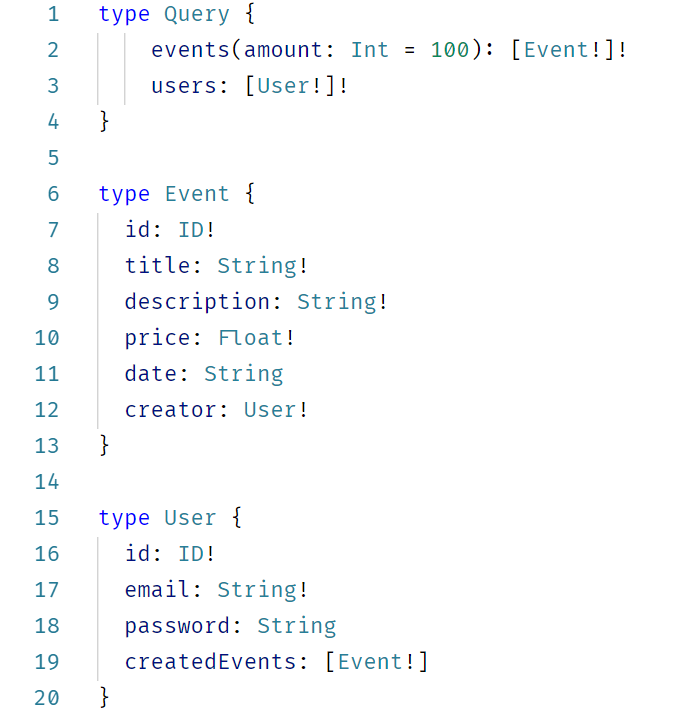
\includegraphics[width=0.6\linewidth]{graphql-schema.png}}
  \caption{GraphQL Beispielschema}\label{code:gql-schema}
\end{figure}

\subsubsection{Abfragen}
Eine GraphQL-Abfrage (Query) beschreibt deklarativ, welche Daten vom Server erwartet werden~\cite[vgl.][]{GraphQL-spec-github}
Üblicherweise beginnt eine Query mit einem der drei Root-Typen, gefolgt von einem optionalen Query-Namen.
Die Abfrage richtet sich nach dem Schema und kann durch die Referenzen zwischen den Typen beliebig tief geschachtelt werden.
Alle Felder, die ein Client erhalten möchte, müssen in der Query angegeben werden.
Queries können mit Variablen parametrisiert werden, damit die sie leichter wiederverwendbar sind und nicht manuell verkettet werden müssen.
Folgende Query könnte auf dem vorangegangenen Schema ausgeführt werden:
\begin{figure}[h]
  \centering
  \fbox{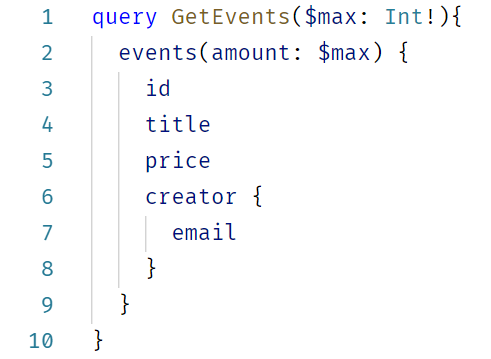
\includegraphics[width=0.5\linewidth]{graphql-query.png}}
  \caption{GraphQL Query}\label{img:graphql-query}
\end{figure}
\par
Die Antwort ist üblicherweise ein JSON-Objekt mit der gleichen Struktur, wie die Abfrage.
\begin{figure}[h]
  \centering
  \fbox{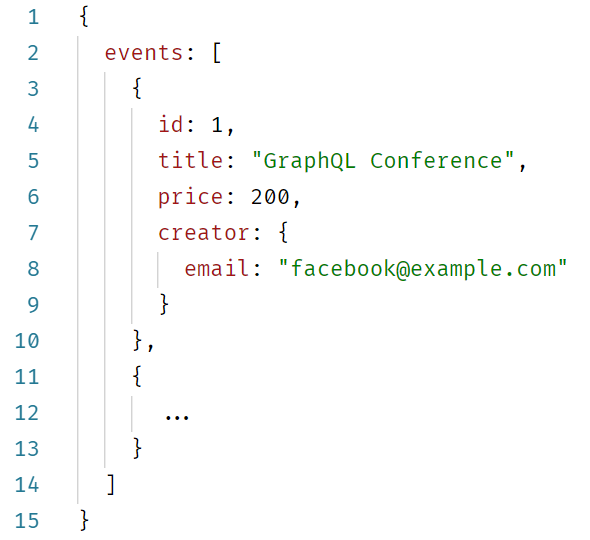
\includegraphics[width=0.6\linewidth]{graphql-query-response.png}}
  \caption{Die Antwort zu~\ref{img:graphql-query}}\label{img:graphql-response}
\end{figure}
\par
Eine GraphQL API ermöglicht Introspektion, d.h.\ dass auf allen Typen spezielle Felder abgefragt werden können, die das Schema selbst und typspezifische Metainformationen zurückgeben.
Diese Eigenschaft kann durch Entwicklungswerkzeuge genutzt werden, um zur Entwicklungszeit automatische Vervollständigung oder statische Validierung der Abfragen anzubieten~\cite[vgl.][]{Postman-GraphQL}
\par
Die GraphQL Spezifikation macht keine Angaben zum Übertragungsprotokoll.
Es ist jedoch durch die meisten Implementierungen über HTTP vorgegeben, dass jede Anfrage mit der HTTP POST Methode und dem Media Type \emph{application/graphql} an eine einzige URI gesendet wird.
Weiterhin antwortet ein GraphQL-Server immer mit dem Status Code 200, wobei die Daten oder eventuelle Fehler im Response Body enthalten sind.
Nach dem Richardson Maturity Model entspräche eine GraphQL-API damit dem Level 0.

\section{Query-Execution}
Die Verarbeitung einer Anfrage auf dem Server geschieht in 5 Schritten:
\begin{enumerate}
  \item Lexing
  \item Parsing
  \item Validierung der Variablen
  \item Aufrufen der Resolver
  \item Validierung der Rückgabewerte
\end{enumerate}
Nachdem eine Query eingegangen ist, wird diese, aufgrund der von GraphQL festgelegten Grammatik, von einem Zeichenstrom in eine Auflistung der GraphQL Tokens umgewandelt~\ref{img:graphql-lexing}.
\begin{figure}[h]
  \centering
  \fbox{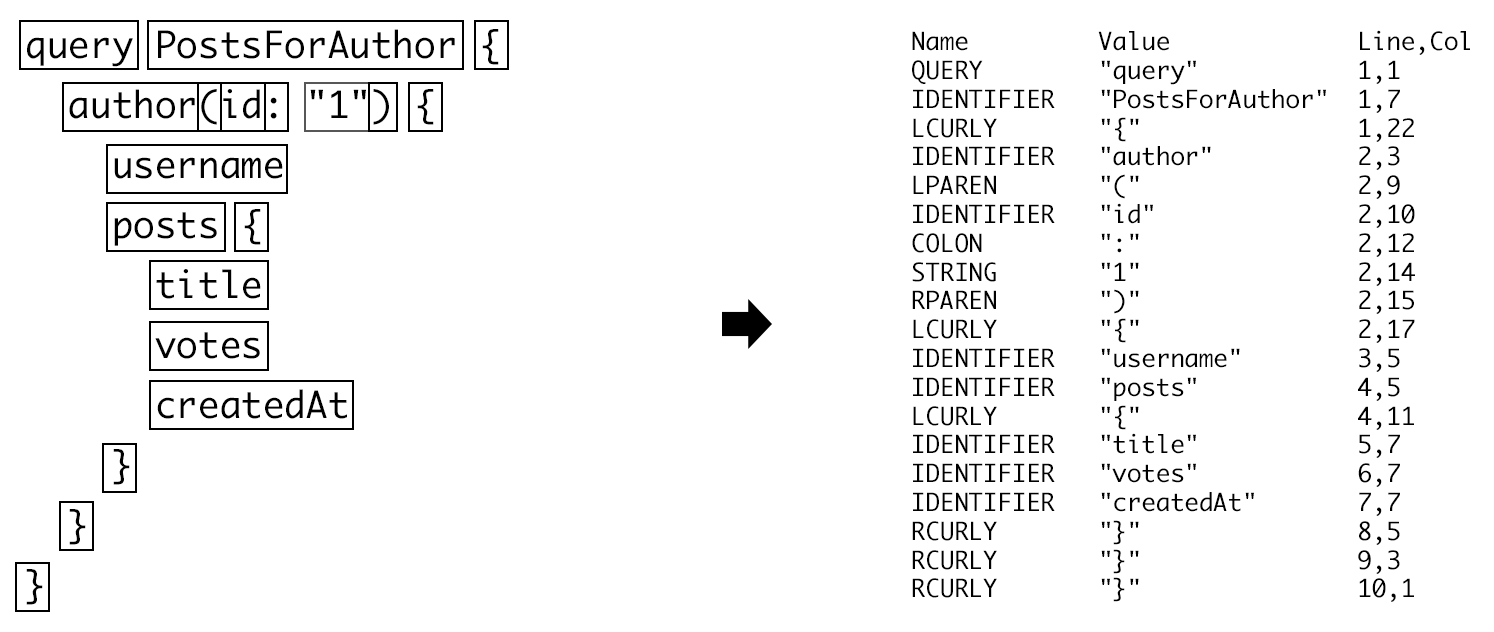
\includegraphics[width=0.9\linewidth]{graphql-lexing.png}}
  \caption{Transformation einer Query durch Lexing~\cite{JoudreyLexParse}}\label{img:graphql-lexing}
\end{figure}
Die Tokens werden anschließend von einem Parser auf strukturelle Richtigkeit geprüft und in einem Abstract Syntax Tree (AST) zusammengefasst, der die Query repräsentiert und schrittweise durchlaufen werden kann, um die Abfrage zu erfüllen~\ref{img:graphql-parsing}.
Der Algorithmus für Lexing und Parsing ist von der GraphQL Spezifikation nicht vorgegeben und kann daher von programmiersprachenspezifischen Datenstrukturen Gebrauch machen bzw.\ verschieden optimiert werden.
\begin{figure}[h]
  \centering
  \fbox{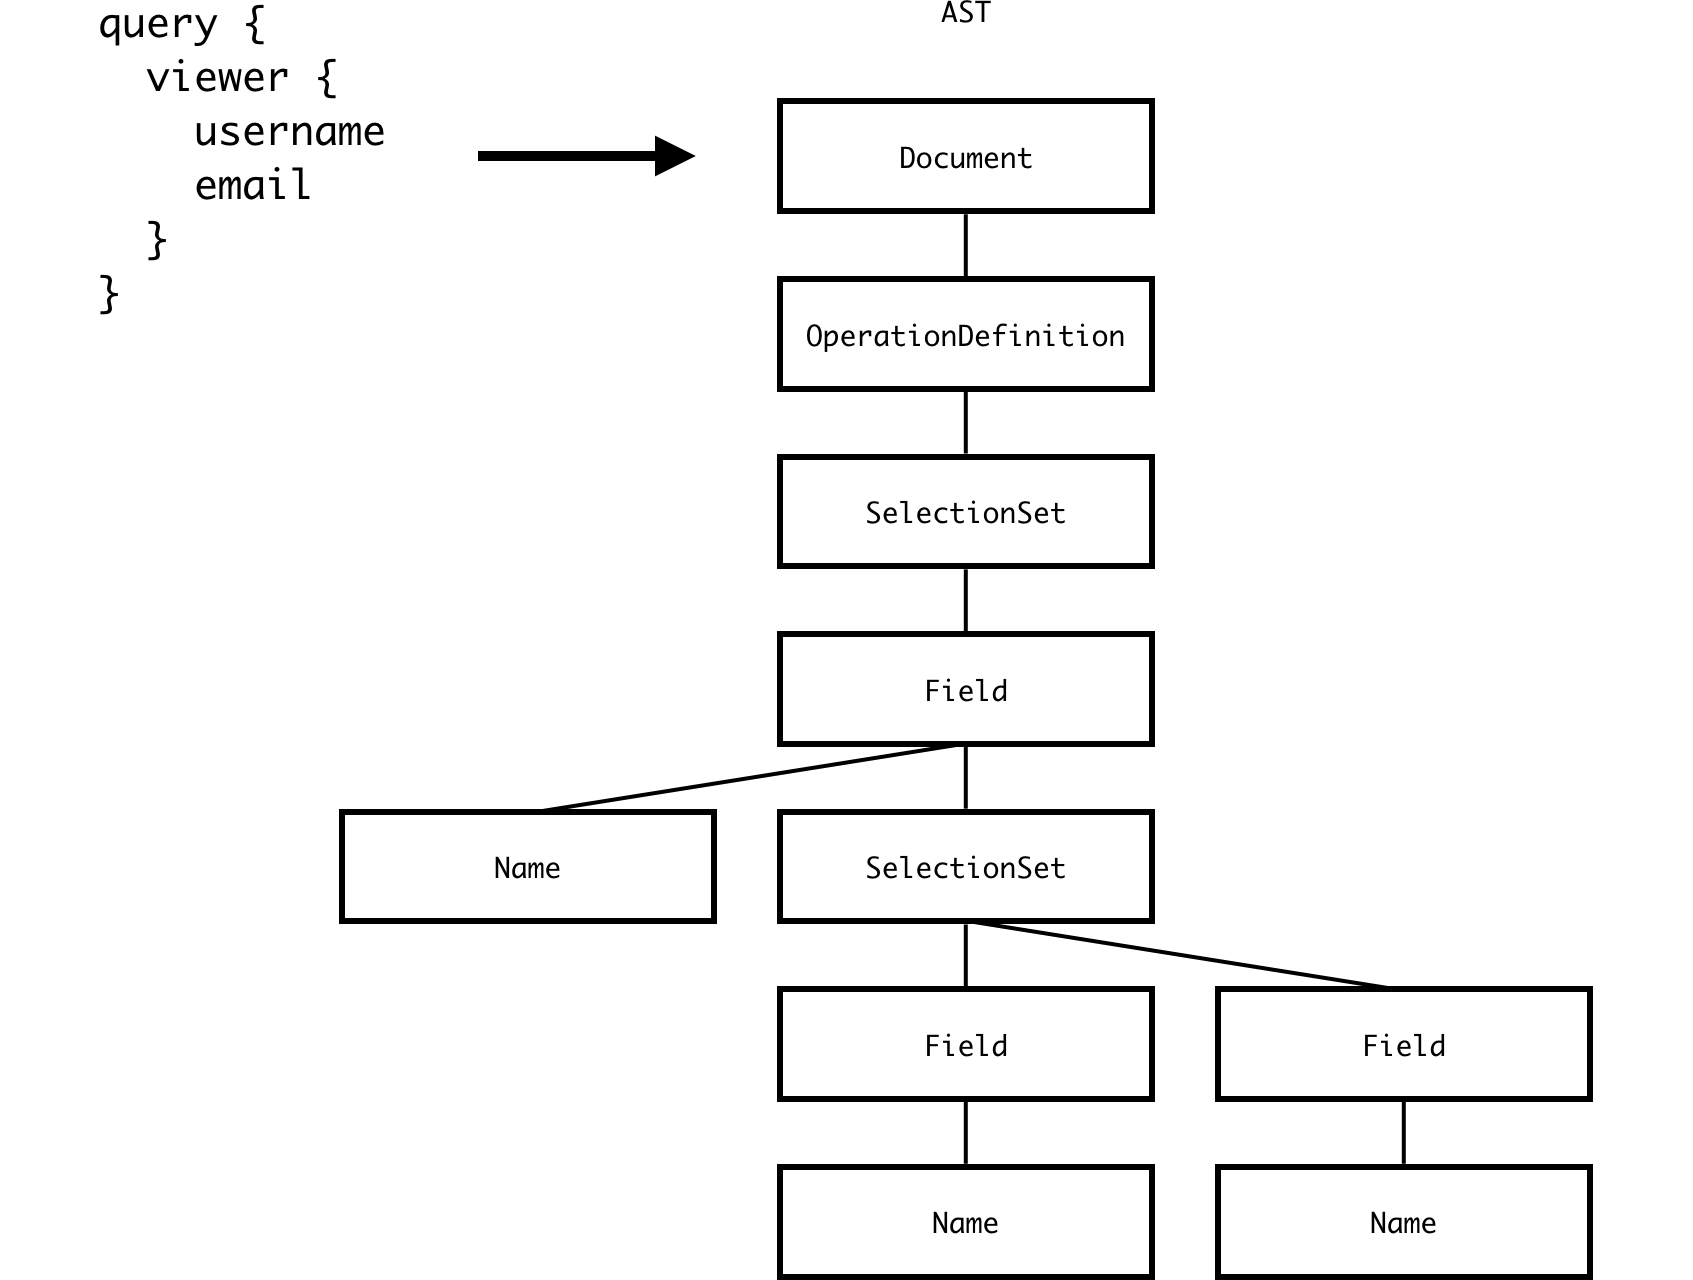
\includegraphics[width=0.7\linewidth]{graphql-ast.png}}
  \caption{Transformation der Query Tokens in den Abstract Syntax Tree~\cite{JoudreyLexParse}}\label{img:graphql-parsing}
\end{figure}
Anhand des AST und des Schemas wird die Abfrage und alle zugehörigen Variablen nach den in der Spezifikation vorgegebenen Regeln validiert~\cite[vgl.][]{JoudreyLexParse}.
Um die gewünschten Daten zu erhalten, muss für jedes Feld ein sogenannter Resolver hinterlegt sein.
Diese Funktion wird aufgerufen und gibt die angefragten Daten zurück.
Es ist für GraphQL dabei transparent, woher die Daten kommen, d.h.\ ein Resolver könnte eine Datenbank oder eine andere API anfragen oder die Daten vom Dateisystem lesen.
Bei einer Query werden die Feldresolver parallel ausgeführt (siehe 3 und 4~\ref{img:graphql-execution}), während sie bei Mutations sequenziell ausgeführt werden.
\begin{figure}[h]
  \centering
  \fbox{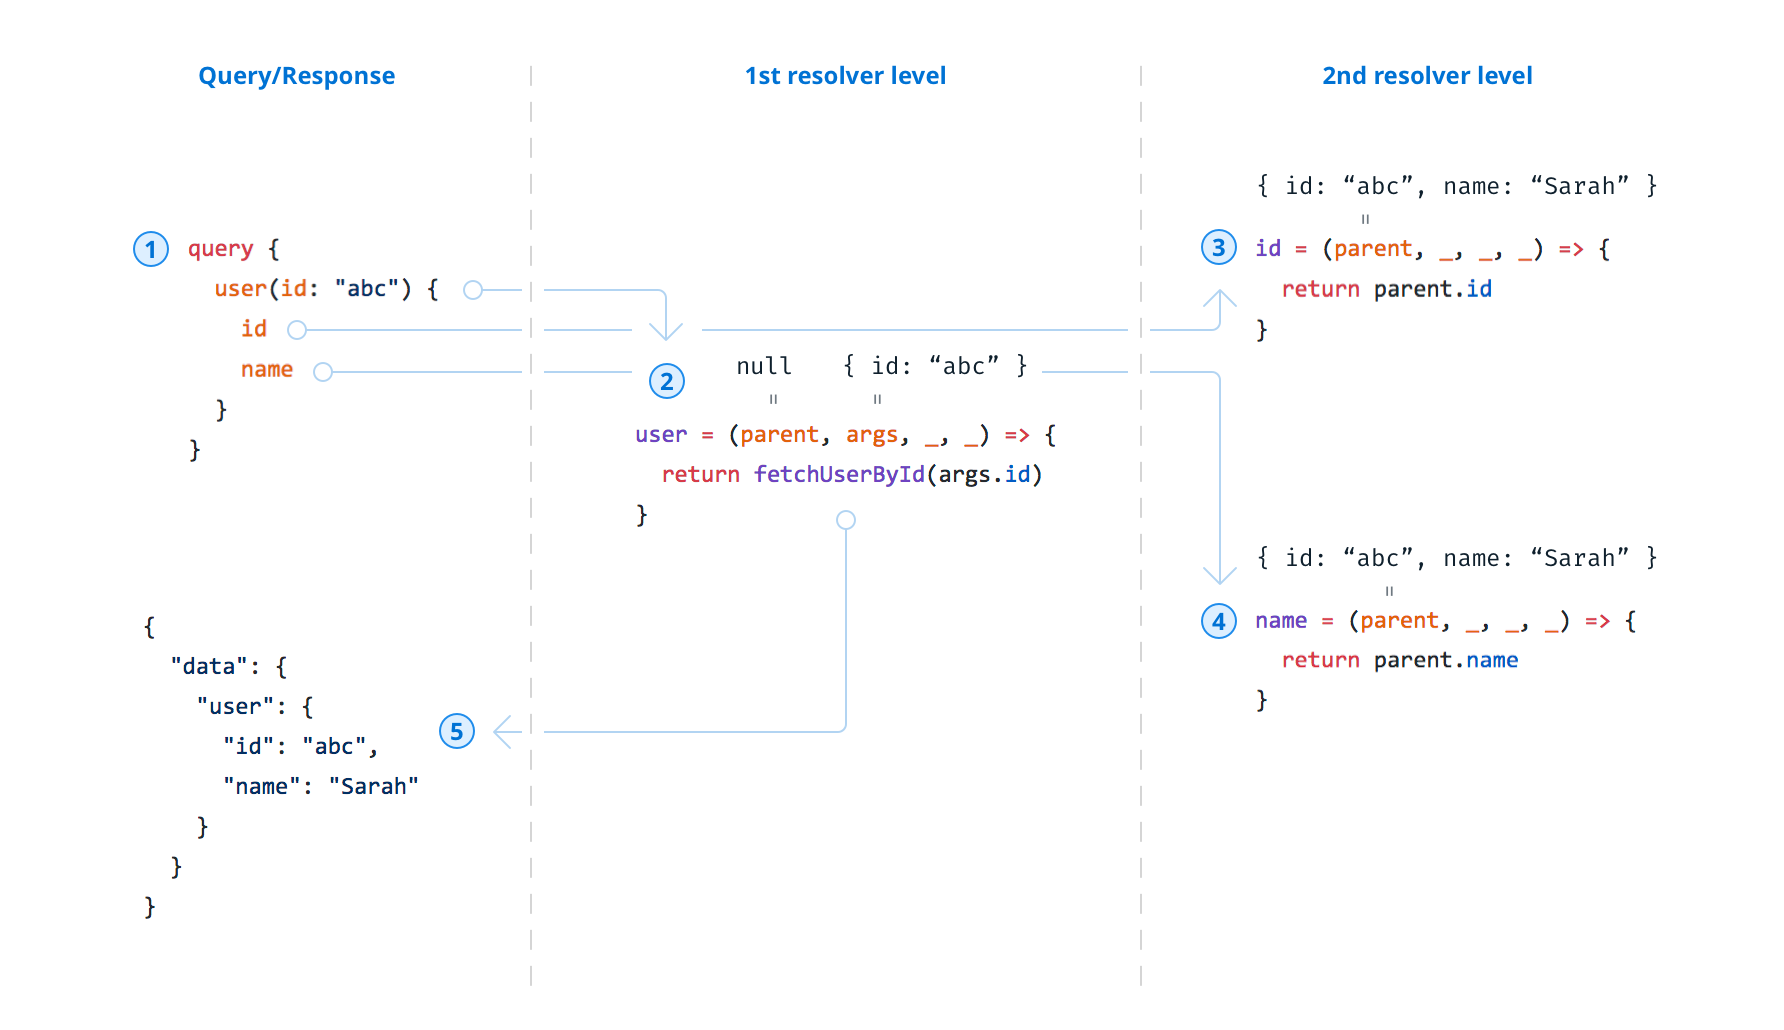
\includegraphics[width=0.8\linewidth]{graphql-query-execution.png}}
  \caption{Aufrufen der Resolverfunktionen~\cite{BurkN}}\label{img:graphql-execution}
\end{figure}
Abschließend werden die Rückgabewerte anhand des Schemas validiert und, falls möglich, in den richtigen Typ konvertiert.
An dieser Stelle zeigt sich ein Nachteil von JSON als Übertragungsprotokoll: GraphQL unterscheidet zwischen Ganzzahlen und Fließkommazahlen, JSON jedoch nicht.
Die Validierung ist notwendig, damit der GraphQL-Server die API erfüllt und nur Daten sendet, die im Schema aufgeführt sind.
